\section{Applications of the IIM}
The IIM has been applied to many varied problems, both linear and non-linear. Some particular examples will be given here, but for a more complete list consult Li and Ito \cite{liito06}.

\subsection{The IIM for electro-migration voiding problems}
Electro-migration voiding problems deal with the movement and deformation of non-conducting voids in thin, metal, current carrying lines such as circuit traces found on the surfaces of printed circuit boards.
This group of problems is part of a larger group of problems dealing with constant volume diffusion along surfaces under the influence of external forces.
For an overview of this class of problems, see \cite{cahntaylor94}.

The solution of electro-migration voiding problems using the IIM is considered in \cite{lizhaogao99}.
Electro-migration voiding problems involve solving a fourth order nonlinear PDE on a rectangular domain.
The IIM is superior to other methods for solving this type of problem for two reasons.
It is less computationally intensive than other methods, and the grid can remain fixed between time steps as opposed to being recalculated after every time step in other methods.
The authors develop a numerical scheme based on the IIM which allows them to numerically model some instances of void migration as show in Figure \ref{EMVDiagram}.

\begin{figure}[h!]
    \centering
    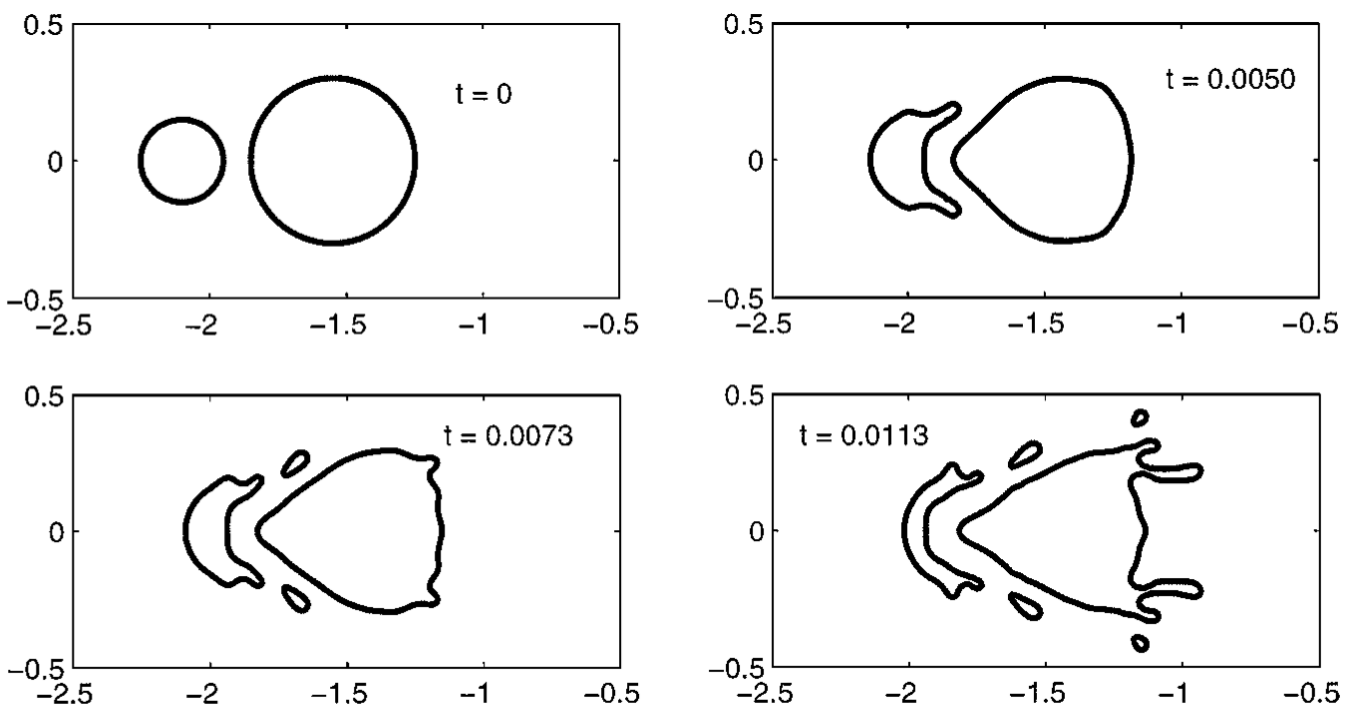
\includegraphics{diagrams/EMVDiagram.png}
    \caption{The simulated evolution of two voids over time. Reprinted from \cite{lizhaogao99}.}
    \label{EMVDiagram}
\end{figure}

\newpage

\subsection{The IIM for electro-capacitance tomography problems}
The IIM has been applied to problems in the field of electro-capacitance tomography (ECT) by considering the IIM in polar coordinates by Alvarez et. al. \cite{alvarezchenli11}.
The usual setup of an ECT machine is a cylindrical tube with some material passing through it.
Around the edges of the tube there are between 8 and 16 electrodes.
Pairs of electrodes are chosen, and the capacitance between them is measured.
This process of choosing pairs of electrodes is repeated until all electrode combinations have been exhausted.

There are two problems of interest in ECT.
The `forwards problem' is to calculate the capacitance that would be measured by electrodes placed around the edges of the ECT machine give a know electromagnetic permittivity inside the device.
The `inverse problem' is to reconstruct the electromagnetic permittivity of the space inside the ECT instrument from a series of capacitance reading by electrodes located around the edge of the device.
ECT is a relatively immature analytical tool, but it has been applied in a few areas including flame monitoring and monitoring of fluidised beds in laboratory tests, and analysis of bead milling and pneumatic conveying processes in industrial tests (\cite{york01} and references therein).
ECT is particularly useful in monitoring mixtures of different materials, because if these materials possess different permittivities, the spatial location of the interfaces between them will be clearly visible in imaging data obtained from ECT machines.

The IIM is a useful tool for solving problems in ECT because the permittivity will have a jump across the interface between different media that are flowing through the ECT device.
Alvarez et. al. \cite{alvarezchenli11} perform a coordinate transformation from cartesian to cylindrical coordinates and set up a numerical scheme for solving the elliptical equation that arises in ECT problems.
The numerical scheme is shown to provide second order convergence against exact results, and numerical experiments are conducted to solve the forwards problem for some given permittivity distributions (see Figure \ref{ECTDiagram}).

\begin{figure}[h!]
    \centering
    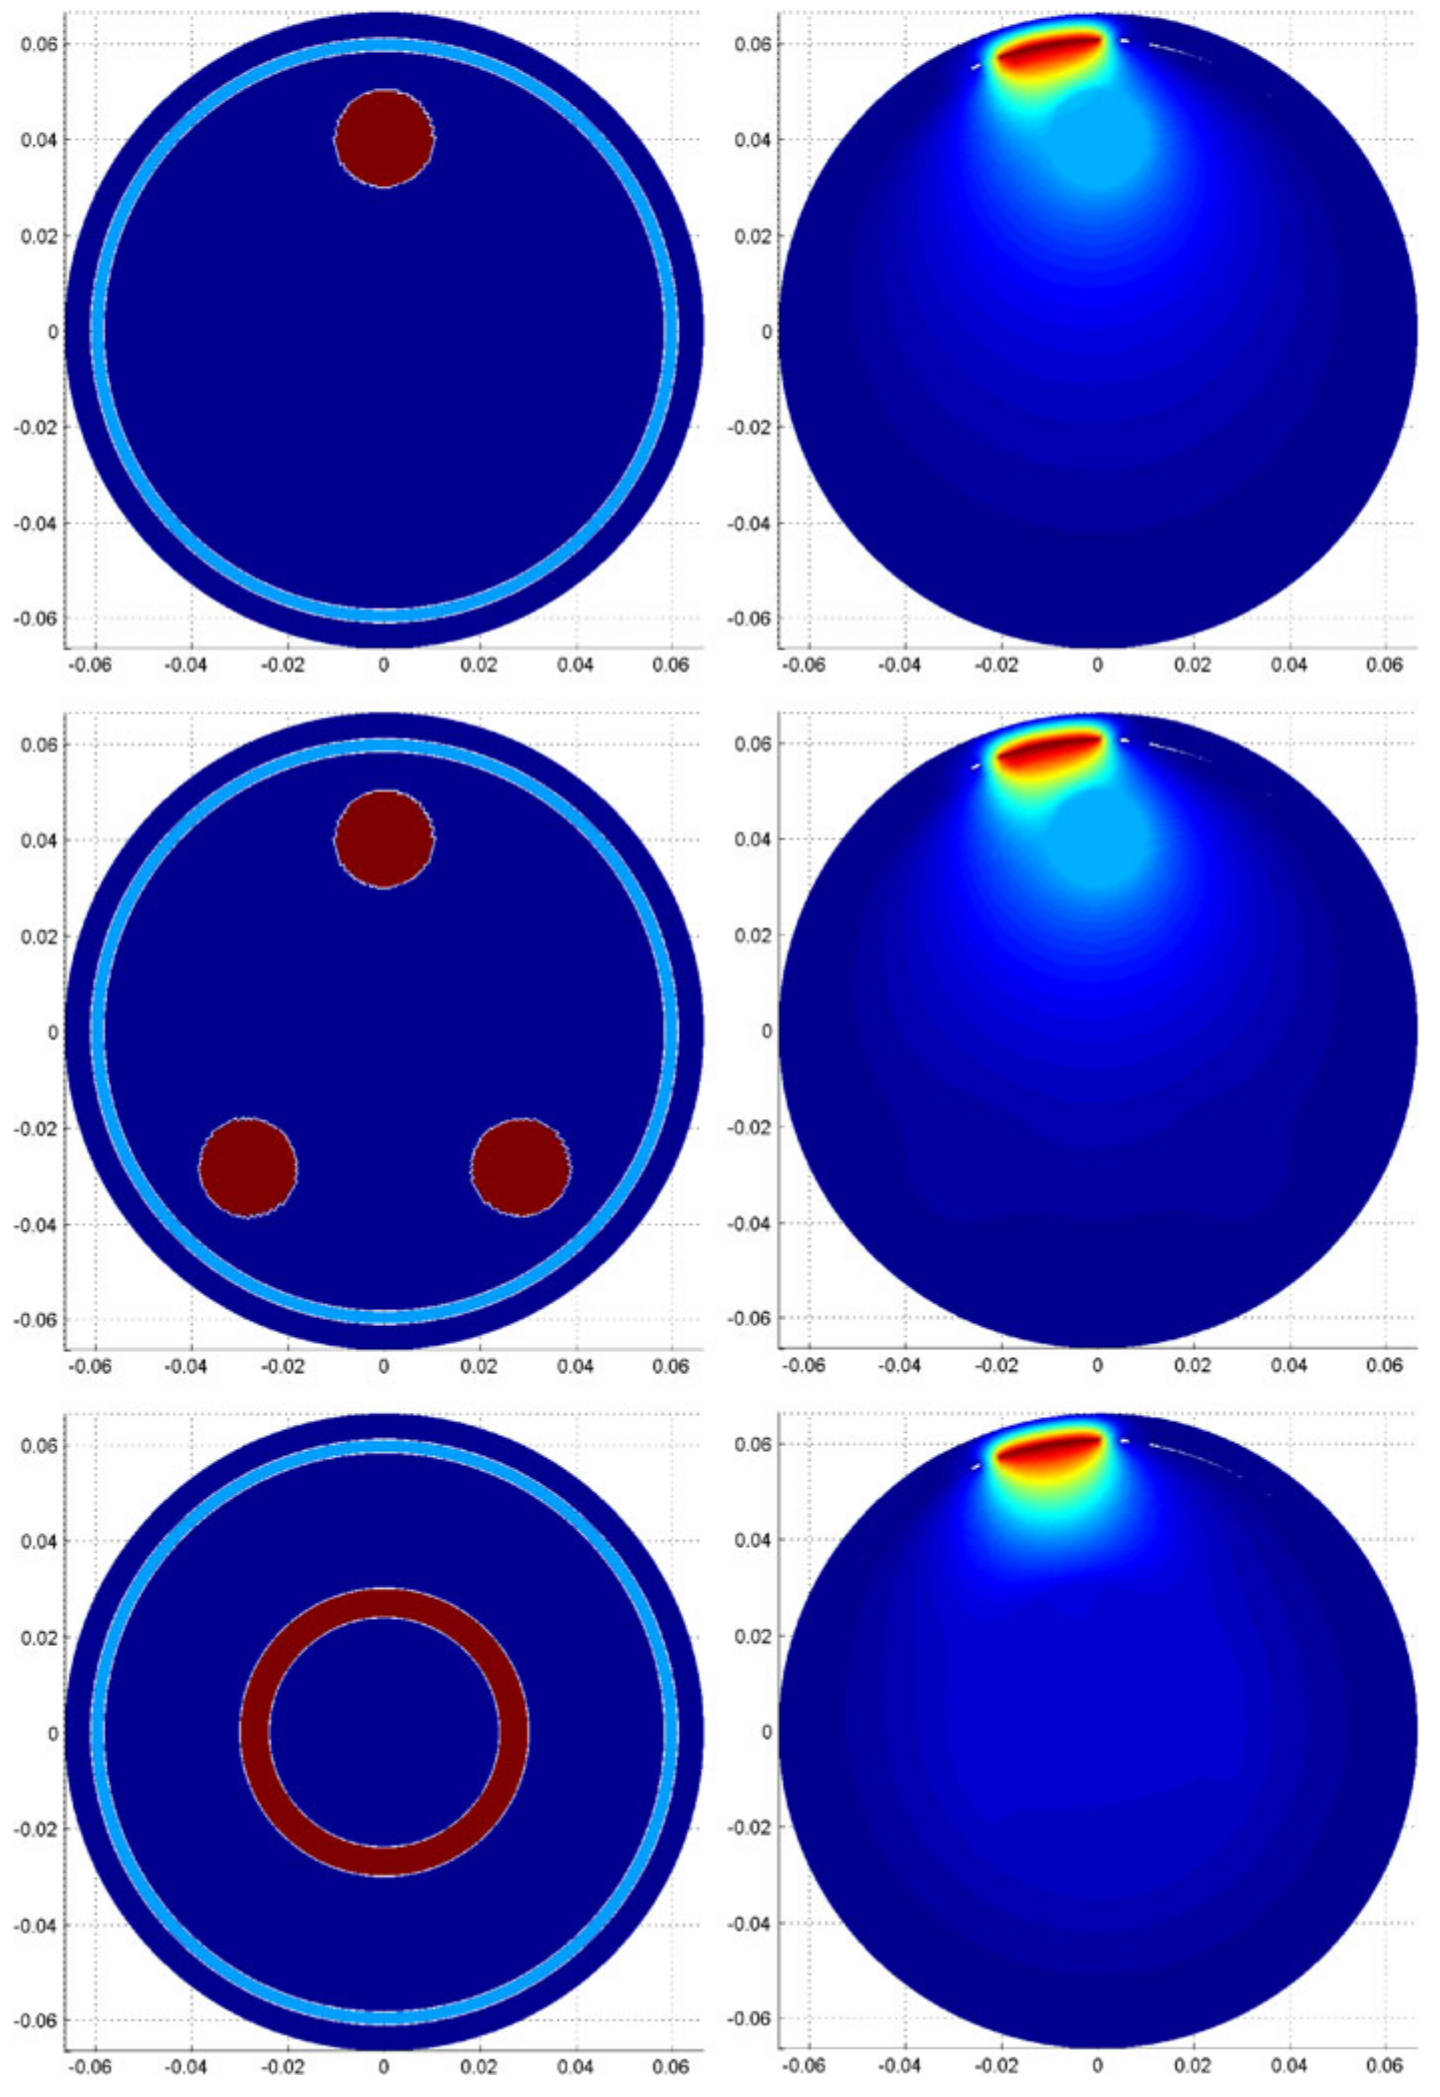
\includegraphics{diagrams/ECTDiagram.png}
    \caption{Solutions (right) calculated from given permittivities (left). Reprinted from \cite{alvarezchenli11}.}
    \label{ECTDiagram}
\end{figure}

\newpage
\clearpage
\subsection{The IIM for traffic flow problems}
The IIM has been used to model problems in traffic flow on highways by Wiegmann and Bube \cite{wiegmannbube98}.
In this paper, the authors develop a model for traffic flow based on some simple assumptions about driver behaviour and conservation of the number of cars.
Discontinuities can arrise in traffic flow problems either due to initial conditions (eg. cars starting from traffic lights) or due to shocks.
The authors begin by confirming that the IIM still retains accuracy when it is used to solve non-linear DEs before modelling a non-linear equations for traffic flow.
An example of the results obtained from this analysis can been seen in Figure \ref{TrafficDiagram}.

\begin{figure}[h]
    \centering
    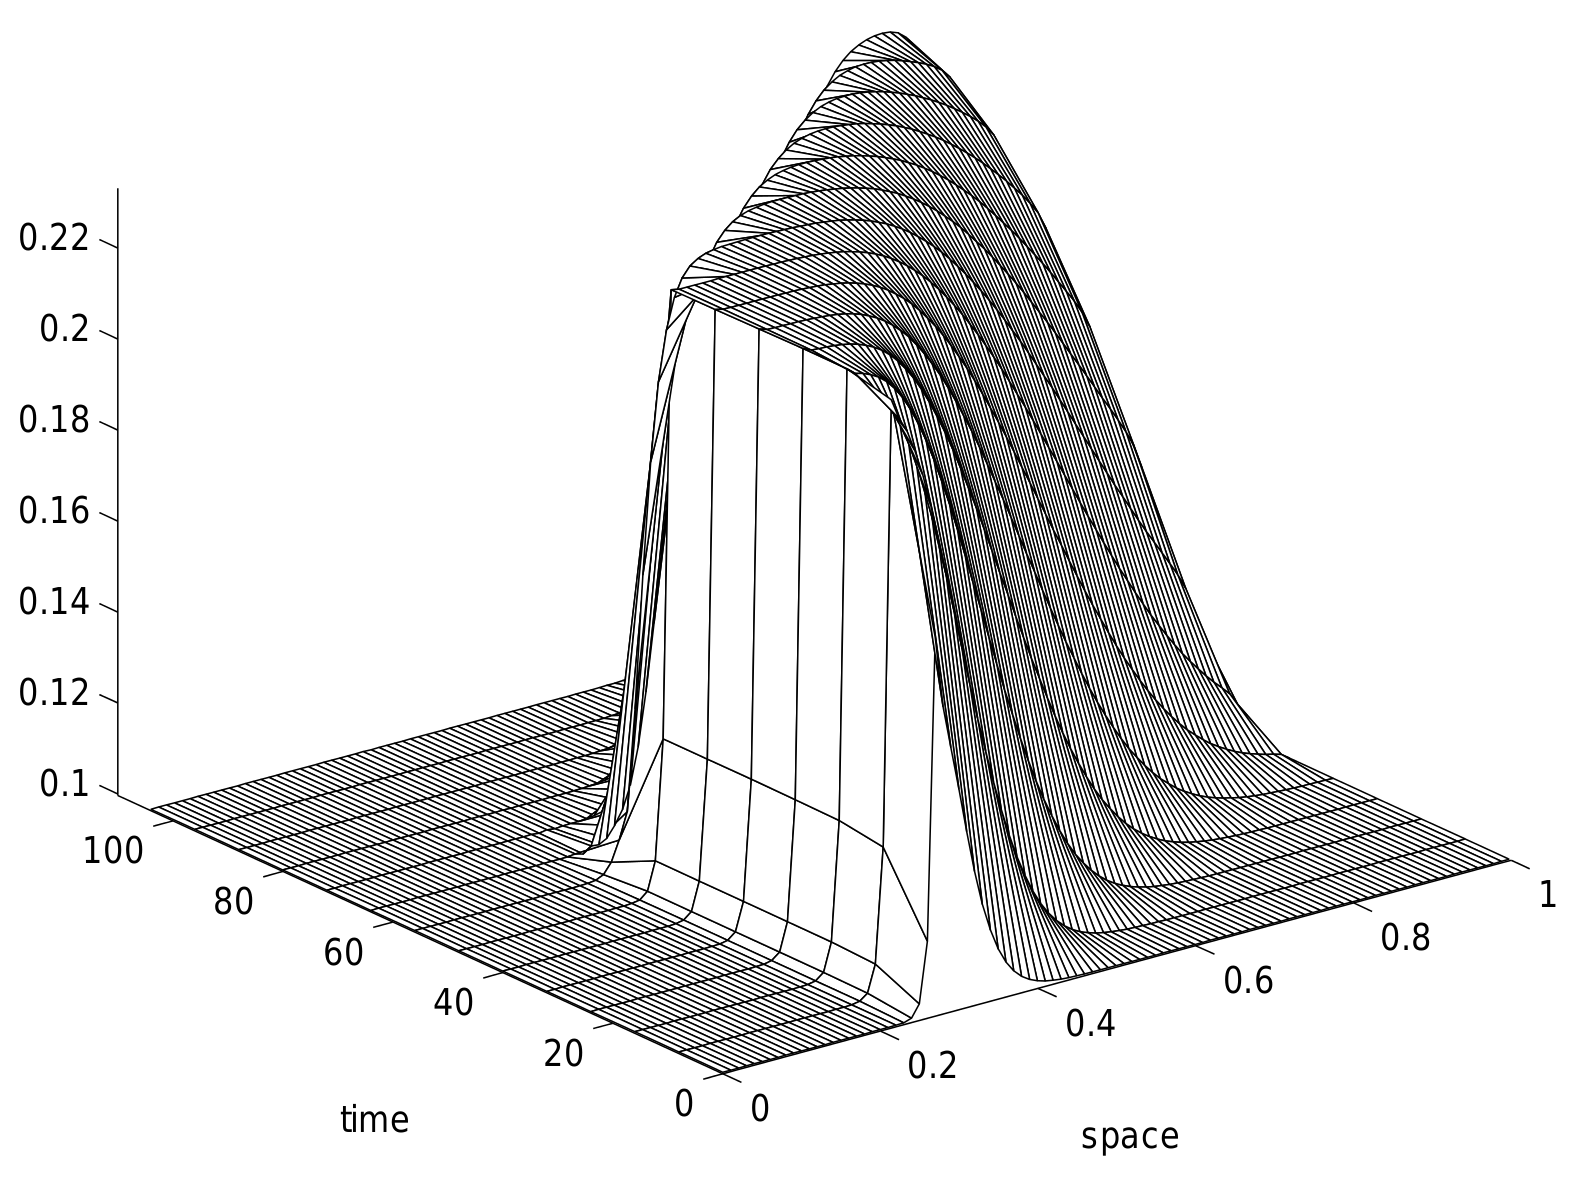
\includegraphics{diagrams/TrafficDiagram.png}
    \caption{A simulation of a constant inbound flow of cars followed by an abrupt stop. The vertical axis here is car density. Note the wave-like propagation of the influx of cars, as well as the diffusion of density away from the congested areas. Reprinted from \cite{wiegmannbube98}.}
    \label{TrafficDiagram}
\end{figure}

\newpage

\subsection{The IIM for crystal growth}
The complex patterns of snowflakes are produced by an interplay between heat diffusion, surface tension and a moving interface.
This makes it an ideal problem to solve using the IIM.
In general, crystal growth problems occur any time a compound is slowly changing phases eg. solid to liquid in the case of a snowflake.
This process involves heat diffusing through the different phases at different rates, as well as heat being generated by the phase change at the boundary and a curvature and surface tension dependant condition at the boundary.
For a more thorough treatment of the subject of crystal growth consult \cite{langer80}.
Li and Soni \cite{lisoni99} use the IIM with both a modified Crank-Nicholson scheme and alternating directional implicit (ADI) method to solve problems of crystal growth.
Some numerical results can be seen in Figure \ref{CrystalDiagram}.

\begin{figure}[h]
    \centering
    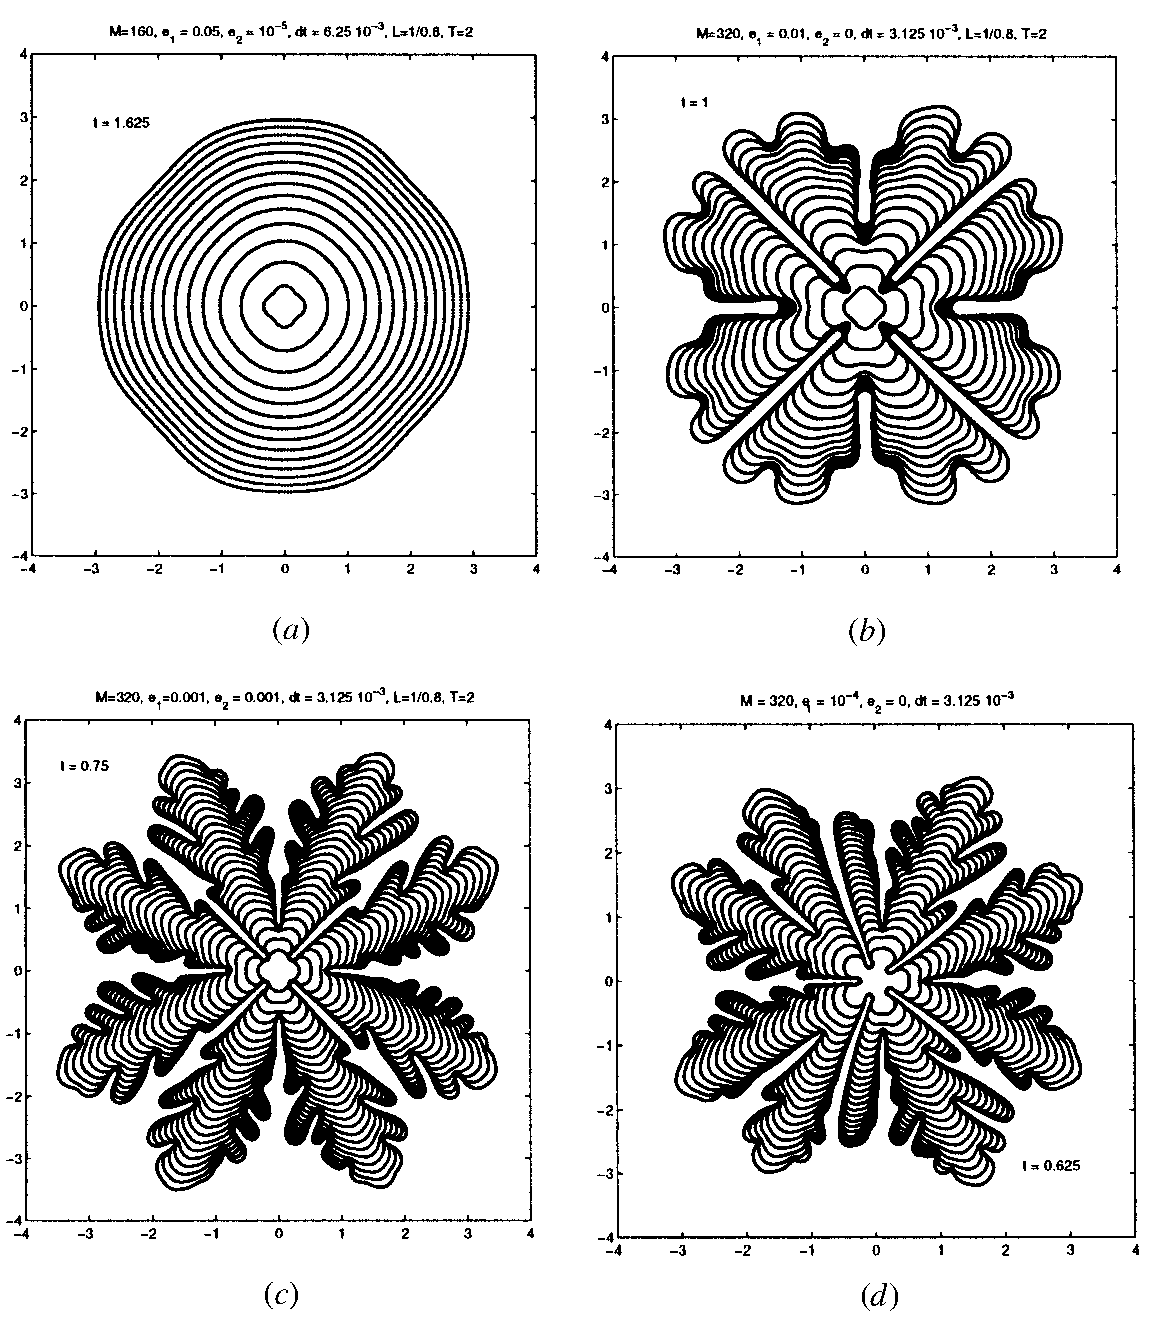
\includegraphics{diagrams/CrystalDiagram.png}
    \caption{Crystal growth with different values for surface tension. The figures are labelled in order of decreasing surface tension. It is evident that lower values of surface tension encourage greater dendrite growth. Reprinted from \cite{lisoni99}.}
    \label{CrystalDiagram}
\end{figure}

\newpage 
\subsection{The IIM for insect flight}

Bergou et. al. \cite{bergouetal07} have use the IIM in conjunction with other methods to study the phenomenon of wing pitch reversal in insect flight.

Wing pitch reversal is a very rapid adjustment of the angle of the wing relative to the direction of airflow (angle of attack) just prior to the upstroke of the insects wing motion.
In \cite{bergouetal07} the authors use the IIM to solve the Navier-Stokes equations governing airflow around the wing by modelling the wing surface as a singular force.
This allows them to calculate the aerodynamic components of the forces applied to the wing during wing pitch reversal.
From the data generated by the IIM and other studies of insect flight, the authors conclude that wing pitch reversal in insects is in fact passive.
That is, no action is required by the insect to cause wing pitch reversal as it is merely a consequence of the aerodynamic force exerted on the wing by the surrounding air.

Figure \ref{wingDiagram} shows a snapshot of the vorticity field as calculated by the IIM, just prior to the rotational motion of wing pitch reversal.

\begin{figure}[h]
    \centering
    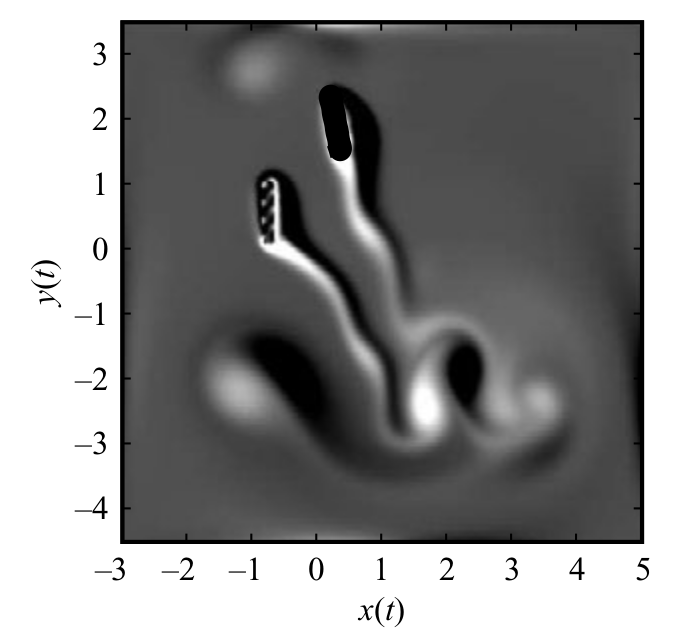
\includegraphics[width=0.5\textwidth]{diagrams/InsectFlight.png}
    \caption{A snapshot of vorticity just prior to rotation of the wing, calculated using the IIM. The dark oval areas in the upper left are the two wings on one side of a dragonfly. Reprinted from \cite{bergouetal07}.}
    \label{wingDiagram}
\end{figure}

